% model.tex -- Methodology: the system model, stated once in the planner's notation.
% Merged 9 Oct (structure audit) from the literature review's payload model (modelling.tex,
% "Cable-Suspended Payload Dynamics") and the planner's model (controller.tex, "Load--cable planner").
% Where the two notations conflicted the planner's is kept. What changed from the review's version:
%  - the rod force T_i is written lambda_i q_i, with q_i pointing from the attachment point to UAV i;
%  - the payload moment is lambda_i rho_i x R_L^T q_i in the payload frame (was rho_i x T_i, frame
%    unstated);
%  - the payload attitude is the quaternion q_L with rotation R_L (was R_L only), and its velocity v_L;
%  - the UAV's equation m_q pddot_i = R_i f_i e3 - m_q g e3 - T_i (scalar thrust f_i along body z) is
%    replaced by the thrust vector f_i each UAV must produce, eq:thrust_req, which is the same equation
%    solved for the thrust; the UAV attitude R_i is then the direction of f_i;
%  - the UAV positions are not states: they follow from the rod kinematics (eq:rod_kin), with the pivot
%    offset delta; the state count is 13 + 14N (the review counted UAV states instead);
%  - a constant force d on the payload is added for steady-error rejection.
% The code (mpc_planner, after Sun et al.) uses s_i = -q_i and t_i = lambda_i.

\subsection{Model and planner}
\label{sec:model}

\subsubsection{System model}

The controller's model follows the load--cable formulation of \cite{tudelft} with the standard
simplifications of Section~\ref{sec:lit_models}: the payload is a rigid body of known mass and inertia,
and each link a rigid, massless rod, taut at all times, whose direction and tension are states. The
formulation calls the links cables, hence the names load--cable planner and cable feedforward (the rod's
planned pull passed to the trackers). The fixed team of the literature
\cite{efficient, wahbaKinodynamicMotionPlanning2024, quan2025swarm} is relaxed so that UAVs can join or
leave mid-flight:
the attachment points and rod lengths are runtime parameters, and the team size selects a solver
(Section~\ref{sec:reconfig}).

The payload has mass $m_L$, inertia $\mathbf{J}_L \in \mathbb{R}^{3\times3}$, position $\mathbf{p}_L$,
velocity $\mathbf{v}_L$, attitude quaternion $\mathbf{q}_L$ (rotation $R_L$) and angular velocity
$\boldsymbol{\omega}_L$ in its own frame. $N$ UAVs pull on it through rods of length $l_i$ attached at
$\boldsymbol{\rho}_i$, offset from the payload's centre of mass (CoM) in the payload frame
(Figures~\ref{fig:geometry} and~\ref{fig:payload_system}). The rod direction $\mathbf{q}_i \in S^2$ points
from the attachment point to UAV $i$, and the rod pulls on the payload with
$\mathbf{T}_i = \lambda_i \mathbf{q}_i$, $\lambda_i \ge 0$.

\begin{figure}[h]
\centering
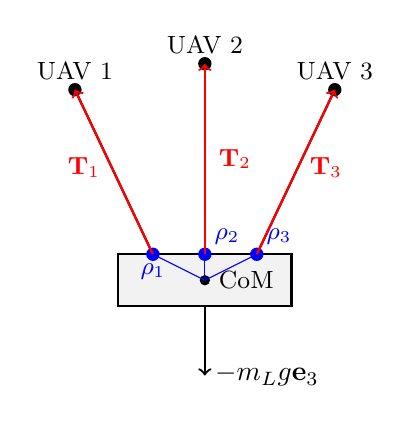
\begin{tikzpicture}[scale=1.1]
  % Payload box
  \draw[thick,fill=gray!10] (-1.0,-0.3) rectangle (1.0,0.3);

  % Centre of mass marker
  \filldraw (0,0) circle (1.5pt);
  \node[right, font=\small] at (0.05,0) {CoM};

  % Gravity
  \draw[->,thick] (0,-0.3) -- (0,-1.1) 
      node[right] {$-m_L g \mathbf{e}_3$};

  % Attachment points on payload surface
  \filldraw[blue] (-0.6,0.3) circle (2pt);
  \filldraw[blue] (0.0,0.3) circle (2pt);
  \filldraw[blue] (0.6,0.3) circle (2pt);

  % UAV 1 - left
  \filldraw (-1.5, 2.2) circle (2pt);
  \node[above, font=\small] at (-1.5,2.2) {UAV 1};
  \draw[thick] (-1.5,2.2) -- (-0.6,0.3);
  \draw[->,red,thick] (-0.6,0.3) -- (-1.5,2.2);
  \node[left, font=\small, red] at (-1.1,1.3) {$\mathbf{T}_1$};
  \draw[->,blue] (0,0) -- (-0.6,0.3) 
      node[below, font=\small, blue] {$\boldsymbol{\rho}_1$};

  % UAV 2 - centre
  \filldraw (0, 2.5) circle (2pt);
  \node[above, font=\small] at (0,2.5) {UAV 2};
  \draw[thick] (0,2.5) -- (0,0.3);
  \draw[->,red,thick] (0,0.3) -- (0,2.5);
  \node[right, font=\small, red] at (0.05,1.4) {$\mathbf{T}_2$};
  \draw[->,blue] (0,0) -- (0,0.3)
      node[above right, font=\small, blue] {$\boldsymbol{\rho}_2$};

  % UAV 3 - right
  \filldraw (1.5, 2.2) circle (2pt);
  \node[above, font=\small] at (1.5,2.2) {UAV 3};
  \draw[thick] (1.5,2.2) -- (0.6,0.3);
  \draw[->,red,thick] (0.6,0.3) -- (1.5,2.2);
  \node[right, font=\small, red] at (1.1,1.3) {$\mathbf{T}_3$};
  \draw[->,blue] (0,0) -- (0.6,0.3)
      node[above right, font=\small, blue] {$\boldsymbol{\rho}_3$};

\end{tikzpicture}
\caption[Multi-UAV payload system]{Multi-UAV payload system: rod $i$ pulls on the payload with tension $\mathbf{T}_i = \lambda_i \mathbf{q}_i$ at the attachment point $\boldsymbol{\rho}_i$, offset from the payload's CoM.}
\label{fig:payload_system}
\end{figure}

Rod $i$ contributes its direction $\mathbf{q}_i$, the angular velocity of that direction $\mathbf{r}_i$
and its first two derivatives, and the tension $\lambda_i$ with its rate:
\begin{equation}
    \mathbf{x} = \big[\, \mathbf{p}_L,\ \mathbf{v}_L,\ \mathbf{q}_L,\ \boldsymbol{\omega}_L,\
    \{\mathbf{q}_i,\ \mathbf{r}_i,\ \dot{\mathbf{r}}_i,\ \ddot{\mathbf{r}}_i,\ \lambda_i,\ \dot{\lambda}_i\}_{i=1}^{N} \,\big]
    \in \mathbb{R}^{13+14N}.
\end{equation}
The inputs are the third derivative of each rod's angular velocity and the second derivative of its
tension, $\mathbf{u} = \{\boldsymbol{\gamma}_i, \eta_i\}_{i=1}^N$, so that the tensions and the rod
directions, and with them the UAV accelerations, are smooth. The dynamics are the payload's
Newton--Euler equations and the rod kinematics:
\begin{align}
    \dot{\mathbf{p}}_L &= \mathbf{v}_L, &
    m_L \dot{\mathbf{v}}_L &= \sum_{i=1}^{N} \lambda_i \mathbf{q}_i - m_L g \mathbf{e}_3 + \mathbf{d},
    \label{eq:plan_trans} \\
    \dot{\mathbf{q}}_L &= \tfrac{1}{2}\, \mathbf{q}_L \otimes \begin{bmatrix} 0 \\ \boldsymbol{\omega}_L \end{bmatrix}, &
    \mathbf{J}_L \dot{\boldsymbol{\omega}}_L &= \sum_{i=1}^{N} \lambda_i\, \boldsymbol{\rho}_i \times R_L^\top \mathbf{q}_i
    - \boldsymbol{\omega}_L \times \mathbf{J}_L \boldsymbol{\omega}_L, \\
    \dot{\mathbf{q}}_i &= \mathbf{r}_i \times \mathbf{q}_i, &
    \dddot{\mathbf{r}}_i &= \boldsymbol{\gamma}_i, \qquad \ddot{\lambda}_i = \eta_i,
\end{align}
where $\mathbf{d}$ is a constant force on the payload, zero in the original formulation and used for
steady-error rejection in Section~\ref{sec:disturbance}. The UAV positions follow from the rod
kinematics,
\begin{equation}
    \mathbf{p}_i = \mathbf{p}_L + R_L \boldsymbol{\rho}_i + l_i \mathbf{q}_i - \boldsymbol{\delta},
    \label{eq:rod_kin}
\end{equation}
with $\boldsymbol{\delta}$ the position of the rod pivot relative to the UAV's
centre ($\boldsymbol{\delta} = -0.04\,\mathbf{e}_3$\,m on the rig). The rod tension couples the system:
it drives the payload in \eqref{eq:plan_trans} and acts, equal and opposite, on UAV $i$.
Differentiating \eqref{eq:rod_kin} twice gives $\ddot{\mathbf{p}}_i$, and the thrust each UAV of mass
$m_q$ must produce is
\begin{equation}
    \mathbf{f}_i = m_q\big(\ddot{\mathbf{p}}_i + g\mathbf{e}_3\big) + \lambda_i \mathbf{q}_i .
    \label{eq:thrust_req}
\end{equation}
The state grows linearly with $N$, which drives the computational scaling noted in \cite{tudelft}.
